% \section{Methods}
\section{Inference}
% \begin{frame}{Graphs}
\label{sec:graph}
Signal transduction network
\begin{itemize}
% graph representation
    \item $\mathcal{G} = \left< \mathcal{V}, \mathcal{E} \right>$
% A signal transduction network in a cell can be represented as a graph $\mathcal{G} = \left< \mathcal{V}, \mathcal{E} \right>$, defined as a set of vertices $\mathcal{V}$ and edges $\mathcal{E}$, where each can be assigned attributes, which often are a single scalar. Typically, an edge connects two vertices (nodes) in a graph and can be either undirected or directed, giving it a source and target node. In a hypergraph an edge can connect more than two nodes, which can be useful for metabolic networks where an edge can represent a reaction, for which there can be multiple input and output metabolites represented as the vertices connected to the edge.
% Edges in a graph representing a protein interaction network can represent the physical binding of proteins or binding of proteins to promotors of genes while nodes represent proteins and genes. Edge attributes can represent regulation strength from TFs to genes, while the node attribute can represent gene product concentration. Genes and their protein products can also be represented as a single node. Separate gene and protein representations are useful if it is not assumed to be known which proteins are coded by which genes. When gene and protein product is a single node ambiguity as to whether an edge is regulating the gene~(transcriptional regulation) or the protein~(protein-protein interaction), can be avoided either with an explicit edge attribute signifying its type of interaction, or by basing the type of interaction on the source node of the edge. The latter can be done if a protein is either strictly classified as a transcription regulator or as a protein regulator. Genes and proteins as separate or combined node representations has both been used in this project. A gene and its protein product were separate in~\autoref{sec:convergence_model}, but otherwise considered a single node.
    \item adjacency matrix
% A Graph can be represented as an adjacency matrix where element $i,j$ is the edge from node $j$ to node $i$. The matrix can be symmetrical, which is used to represent an undirected graph where each element represents the connection between two nodes, without influence from choice in $j$ and $i$. Examples of matrices that can be used as a adjacency matrix representation of an undirected graph are covariance, correlation, and partial correlation matrices.

% If the values are restricted to the Boolean case, for instance ones and zeros, it is used for indication of the presence and absence of an edge. Edges with values -1, 0, and 1 can be used to indicate repression, no effect, and activation, respectively. Real value numbers can encode the strength of activation or repression as well. Positive real value numbers can also be used to indicate weighted edges, for instance representing some concept of attraction forces.
\end{itemize}
DAG
\begin{itemize}
    \item paths can be followed to completion
% Directed Acyclic Graphs (DAGs) are a well studied type of graph, used in fields such as machine learning. When a graph is acyclic and directed there exists no path from a node back to itself, that follows the direction of edges. For this reason it is possible to follow any path to completion. Machine learning networks, such as a feedforward network, will be DAGs with a natural progression layer by layer without infinite loops occurring. This makes it possible to define gradients fully describing how each parameter of a model has influence on the value of network outputs in the last layer of the network.
    \item gene regulation is cyclic
% A biological network modelling transcription and translation relies heavily on feedback loops through the transcription and translation of proteins that regulate other iterations of transcription and translation themselves.
% The cycles complicates many aspects of studying the graph, such as describing conditional independence among the nodes~\cite{Tillman2014}.
\end{itemize}
Network inference
% node inference
% Inferring attributes for the vertices of a biological network can be difficult since attributes such as protein or mRNA concentration generally vary a lot depending on cell cycle and environmental factors. Vertex attributes of interest can be the production level or potential production level of a compound for which we are trying to optimize production.
% edge inference
% Inferring the edges of a biological network is an attempt to understand which protein-protein and protein-DNA interactions are taking place, which should be more static than vertex attributes and is what is usually the focus of biological network inference.
% Wanting to find the edges in the network is to say that we are interested in causal connections. As opposed to typical machine learning training of prediction networks we are not interested in finding a nonlinear function mapping from an input to an output as well as possible with a black-box method, but instead to use biological data to shape the causal edges in a network. Predictive performance can however be a secondary objective.
\begin{itemize}
    \item Likelihood based
% Graph learning has been explored using methods maximizing likelihood. Functions are described for the probability of a set of graph edges given observed attributes of the network, and the optimal graph is selected. There are many benefits to a likelihood based approach to edge inference, where the model will describe the basis for inferences and the confidence in them, compared to for instance a "black box" machine learning approach.
% There are also issues with the complexity of likelihood approaches, where graphs with different edges can have equal likelihood of fitting a given dataset, edges might not indicate causality, the amount of data required for a convergent solution grows exponentially with the number of parameters to infer, and heuristics are usually applied to find suboptimal solutions as discussed by Yeang~\cite{Yeang2004}. Yeang goes on to describe and test a model for graph inference where edges are inferred to be present or absent, and if present, inferred to have positive or negative effects of target nodes. The edge strength is used as a p-value to evaluate certainty of predictions. The model is based on log likelihood ratios for hypothesis testing on graph parameters. Knockout data are applied, and the model constrained by protein-protein interaction data and protein-DNA interactions.
\cite{Yeang2004}
% We will combine similar data here, and also use the absolute sizes of predicted edge weights as a score for our belief in the presence in an edge in the graph.
\end{itemize}
\end{frame}


\subsection{Causality and cyclic graphs}
\begin{frame}{Causality and cyclic graphs}
\label{sec:eberhardt}
\begin{columns}
\begin{column}{0.65\textwidth}
% Causal structure learning, where causal edges are inferred on graphs representing real systems, is often performed on DAGs, as described in a review by Heinze-Deml~et~al.~\cite{CausalLearningReview}. DAGs are too simple to use for biological networks where gene transcription products are taken into account. The only model in the review that is designed for cyclic graphs is BackShift, which is an extension of LLC~(Linear, Latents, Cyclic) described by Eberhardt~et~al.~\cite{EberhardtLLC}. Both methods are designed in pursuit of inferring network edges from node attributes observed under different interventions. The interventions are changes to nodes in the graph, which breaks all ingoing edges. In LLC it is assumed to be known which nodes have been intervened on, which is not assumed with BackShift. For knockout studies we know which nodes (genes) have been knocked out, so LLC is discussed here.
% We first assume a system of node values that are controlled linearly by the values from all parent nodes through discreet time steps~(\autoref{eq:eber_linear}).
Eberhardt et al.~\cite{CausalLearningReview}
\begin{subequations}
\label{eq:eber_linear}
\begin{align}
x_i (t) &=
    \sum_j b_{ij} x_j (t - 1) + e_i
\\
\label{eq:eber_linear.b}
\boldsymbol{x}(t) &=
    B \boldsymbol{x} (t - 1) + \boldsymbol{e}
=
    B \left( B \boldsymbol{x} (t - 2) + \boldsymbol{e} \right) + \boldsymbol{e} = ...
\\
&=
    B^t \boldsymbol{x}(0) + \sum_{i=0}^{t-1} B^i \boldsymbol{e}
\label{eq:eber_time.b}
\\
\lim_{t \rightarrow \infty} B^t &= 0
\quad,\quad
\lim_{t \rightarrow \infty} \sum_{i=0}^{t-1} B^i = \left( I - B \right)^{-1}
\qquad\qquad\qquad\text{\cite{Fisher1970}}
\label{eq:eber_converge}
\end{align}
\end{subequations}
% $e_i$ is added as a term to describe latent variables and noise. Latent variables are any hidden variables in the network not included in $\boldsymbol{x}(t)$.
% We can imagine how this generalizes to any time $t$ relative to the start time $t=0$~(\autoref{eq:eber_time}).
% Having cycles in the model means there can be infinite loops of regulation so to capture all regulation effect for cycles in the model $t$ has to tend to infinity. We first have to assume that $\boldsymbol{x}(t)$ converges for $t\rightarrow \infty$. A realistic system is not expected to diverge. Microorganism have exponential growth hindered only by outside factors that we are not considering in the model, but the growth is exponential due to unhindered cell division, but we assume that there is no exponentially increasing level of synthesis inside the cell, and we only model the workings inside a single cell. There is of course another option which is that $\boldsymbol{x}(t)$ fluctuates or in another way neither converges to an equilibrium nor diverges to infinity. Eberhardt~et~al. also considers this and proofs that the conditions for the model can be extended to accept semi-stable systems.
% Each of the two terms defining $\boldsymbol{x}(t)$~(\autoref{eq:eber_time.b}) are found without restriction on $\boldsymbol{x}(0)$ and $\boldsymbol{e}$ when $t$ tends to infinity~(\autoref{eq:eber_converge}):
% The equations hold when all eigenvalues $\lambda_k$ of $B$ satisfies $|\lambda_k| < 1$~\cite{Fisher1970}. The notation with indication of time is dropped when equilibrium is reached:
Equilibrium
\begin{subequations}
\label{eq:eber_simple}
\begin{align}
\lim_{t \rightarrow \infty} \boldsymbol{x}(t) = \boldsymbol{x} &=
    \left( I - B \right)^{-1} \boldsymbol{e}
\\
\left( I - B \right) \boldsymbol{x} &=
    \boldsymbol{e}
\\
\boldsymbol{x} &=
    B \boldsymbol{x} + \boldsymbol{e}
\end{align}
\end{subequations}
\end{column}
\begin{column}{0.35\textwidth}
\begin{figure}[ht]
    \centering
    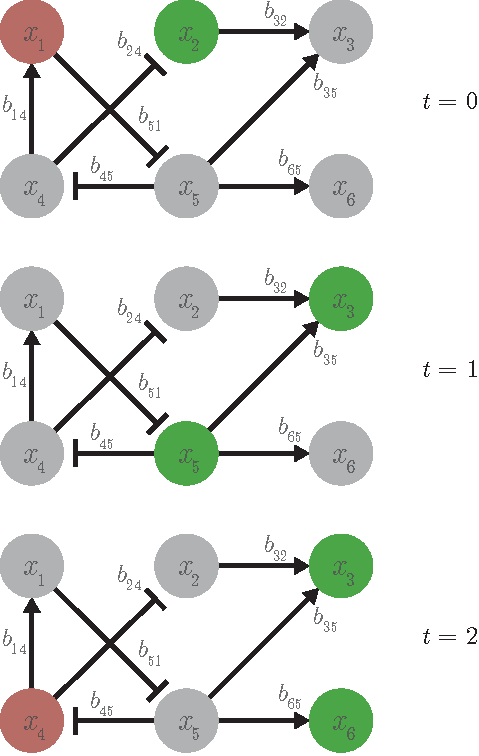
\includegraphics[width=.8\textwidth]{theory/fig/eberhardt.pdf}
    \caption{\textbf{Graph with constant edges.} \\ \textcolor{gray}{Gray} = 0, \textcolor{red!60!black}{red} < 0, \textcolor{green!45!black}{green} > 0.}
    \label{fig:eberhardt}
\end{figure}
\end{column}
\end{columns}
\end{frame}
\begin{frame}{Causality and cyclic graphs - Intervention}
\begin{columns}
\begin{column}{0.65\textwidth}
% We see that the convergence values are defined without referencing the node values at $t=0$ and the expression otherwise exactly matches~\autoref{eq:eber_linear.b}, except that taking a step forward or backward in time does not change the node values anymore.

% The diagonal of $B$ describes edges from nodes onto themselves, self-loops. These are unidentifiable from equilibrium data, since it is impossible to tell the difference between an node with a strong activator and a node with a weaker activator but a strong self-loop only based on steady-state gene expression levels. For this reason the diagonal of $B$ is always set to zeros. 

% The model is then expanded to include a concept of intervention of variables which in the context of biological network experiments is the equivalent of a knockout experiment of one or more genes. The intervention is the replacement of a node with a new value that follows standard Gaussian noise independent of the other variables in the network~(\autoref{eq:eber_intervention}).
Intervention
\begin{subequations}
\label{eq:eber_intervention}
\begin{align}
\boldsymbol{x}_k(t) &=
    U_k B \boldsymbol{x}_k(t-1) + U_k \boldsymbol{e} + \boldsymbol{c}_k
\\
\lim_{t \rightarrow \infty} \boldsymbol{x}_k(t) = \boldsymbol{x}_k &=
    (I - U_k B)^{-1} (U_k \boldsymbol{e} + \boldsymbol{c}_k)
\\
(I - U_k B) \boldsymbol{x}_k &=
    U_k \boldsymbol{e} + \boldsymbol{c}_k
\\
\label{eq:eber_intervention.d}
\boldsymbol{x}_k &=
    U_k B \boldsymbol{x}_k + U_k \boldsymbol{e} + \boldsymbol{c}_k
\end{align}
\end{subequations}
\end{column}
\begin{column}{0.35\textwidth}
\begin{figure}
    \centering
    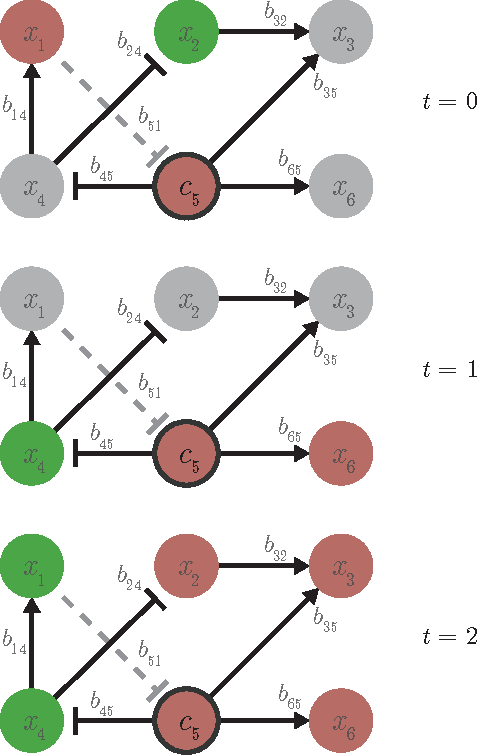
\includegraphics[width=.8\textwidth]{theory/fig/eberhardt_intervention.pdf}
    \caption{\textbf{Intervention on $x_5$.} \\ \textcolor{gray}{Gray} = 0, \textcolor{red!60!black}{red} < 0, \textcolor{green!45!black}{green} > 0.}
    \label{fig:intervention}
\end{figure}
\end{column}
\end{columns}
\end{frame}

\begin{frame}{Causality and cyclic graphs - $E[\boldsymbol{x}_k]$, covariance, and variable separation}
% The noise is given in $\boldsymbol{c}_k$ for the $k$-th experimental setup, where every value is zero except at the indexes of intervened nodes in experimental setup $k$. We refer to $k$ as an experimental setup rather than simply as an experiment to make it clear that the $k$-th experimental setup can be repeated multiple times, creating multiple observations of $\boldsymbol{x}_k$. The effect of other nodes onto the intervened variable is completely removed. 
% This makes sense in terms of a knockout where a removed gene will no longer be regulated by TFs. This is modelled using $U_k$ which is a diagonal matrix of ones, except at the indexes of intervened variables in experiment~$k$, where it has a value of zero. The result is the complete removal of the corresponding rows of $B$ and elements of $\boldsymbol{e}$. 
% A covariance matrix can be estimated if there are multiple observations for each experiment setup~$k$~(\autoref{eq:eber_cov}).
Expectation and covariance
\begin{subequations}
\label{eq:eber_cov}
\begin{align}
E[\boldsymbol{x}_k] &= (I-U_kB) ^{-1} \mu_{\boldsymbol{c}_k}
\\
\Sigma_{\boldsymbol{x}_k}
&=
\E \left[(\boldsymbol{x}_k - \E[\boldsymbol{x}_k] )(\boldsymbol{x}_k - \E[\boldsymbol{x}_k])^\trans \right]
\\
&= (I-U_kB)^{-1} E\left[ (U_k\boldsymbol{e}_k + \boldsymbol{c}_k - \mu_{\boldsymbol{c}_k})(U_k\boldsymbol{e}_k + \boldsymbol{c}_k - \mu_{\boldsymbol{c}_k})^\trans \right] (I-U_kB)^{-\trans}
\\
&= (I-U_kB)^{-1} (\Sigma_{\boldsymbol{c}_k} + U_k\Sigma_{\boldsymbol{e}} U_k) (I-U_kB)^{-\trans}
\end{align}
\end{subequations}
% Where $\mu_{\boldsymbol{c}_k}$ is the expected value of $\boldsymbol{c}_k$, and $\Sigma_{\boldsymbol{x}_k}$ is the covariance matrix of $\boldsymbol{x}_k$. The interesting parts of the covariance matrix are the entries describing covariance between the intervened variables and the passively observed variables. Since it is assumed that no variable has an effect onto intervened variables it can be possible to describe the observed covariance as more than just an undirected covariance edge between the two nodes but instead as a directed edge of causality from the intervened to the non-intervened.
% We denote the elements of vectors and matrices with subscript $\mathcal{J}_k$, $\mathcal{U}_k$, and $\mathcal{V}$ to refer to indexes for nodes intervened on in experimental setup $k$, passively observed in experimental setup $k$ and indexes of all nodes, respectively. We split our expression for $\boldsymbol{x}_k$ from \autoref{eq:eber_intervention.d} into expressions for intervened and non-intervened variables~(\autoref{eq:JU}).
Separating intervened ($\boldsymbol{x}_{\mathcal{J}_k}$) and passively observed ($\boldsymbol{x}_{\mathcal{U}_k}$) variables
\begin{subequations}
\label{eq:JU}
\begin{align}
\boldsymbol{x}_{\mathcal{J}_k} &= \boldsymbol{c}_{\mathcal{J}_k}
\\
\boldsymbol{x}_{\mathcal{U}_k} &= B_{\mathcal{U}_k\mathcal{V}} \boldsymbol{x}_k + \boldsymbol{e}_{\mathcal{U}_k}
\\
&= B_{\mathcal{U}_k\mathcal{U}_k} \boldsymbol{x}_{\mathcal{U}_k} + B_{\mathcal{U}_k\mathcal{J}_k} \boldsymbol{x}_{\mathcal{J}_k} + \boldsymbol{e}_{\mathcal{U}_k}
\\
(I - B_{\mathcal{U}_k\mathcal{U}_k}) \boldsymbol{x}_{\mathcal{U}_k} &=
B_{\mathcal{U}_k\mathcal{J}_k}\boldsymbol{x}_{\mathcal{J}_k} + \boldsymbol{e}_{\mathcal{U}_k}
\\
\boldsymbol{x}_{\mathcal{U}_k} &=
(I - B_{\mathcal{U}_k\mathcal{U}_k})^{-1}(B_{\mathcal{U}_k\mathcal{J}_k}\boldsymbol{x}_{\mathcal{J}_k} + \boldsymbol{e}_{\mathcal{U}_k})
\end{align}
\end{subequations}
\end{frame}

\begin{frame}{Causality and cyclic graphs - Covariance between $\boldsymbol{x}_{\mathcal{J}_k}$ and $\boldsymbol{x}_{\mathcal{U}_k}$}
% The covariance between $\boldsymbol{x}_{\mathcal{J}_k}$ and $\boldsymbol{x}_{\mathcal{U}_k}$ can then be described~(\autoref{eq:causal_cov}).
Covariance between intervened ($\boldsymbol{x}_{\mathcal{J}_k}$) and passively observed ($\boldsymbol{x}_{\mathcal{U}_k}$) variables
\begin{subequations}
\label{eq:causal_cov}
\begin{align}
(\Sigma_{\boldsymbol{x}_k})_{\mathcal{J}_k\mathcal{U}_k} &=
\E \left[ (\boldsymbol{x}_{\mathcal{J}_k} - \E[\boldsymbol{x}_{\mathcal{J}_k}])
(\boldsymbol{x}_{\mathcal{U}_k} - \E[\boldsymbol{x}_{\mathcal{U}_k}])^\trans \right]
\\
&= \E \left[
(\boldsymbol{x}_{\mathcal{J}_k} - \E[\boldsymbol{x}_{\mathcal{J}_k}])
(B_{\mathcal{U}_k\mathcal{J}_k} (\boldsymbol{x}_{\mathcal{J}_k} - \E[\boldsymbol{x}_{\mathcal{J}_k}]))^\trans
\right]
(I - B_{\mathcal{U}_k\mathcal{U}_k})^{-\trans}
\\
&= (\Sigma_{\boldsymbol{c}_k})_{\mathcal{J}_k\mathcal{J}_k} B^\trans_{\mathcal{U}_k\mathcal{J}_k} (I - B_{\mathcal{U}_k\mathcal{U}_k})^{-\trans}
\end{align}
\end{subequations}
% Eberhardt~et~al. deals with what they call canonical experiments to simplify notation where each element in $\boldsymbol{c}_k$ is uncorrelated with zero mean and unit variance. From this and the symmetry of covariance matrices we get expression for covariance between intervened and passively observed that only depend on entries of $B$~(\autoref{eq:eberhardt_cov}). Matrix $T_{\boldsymbol{x}_k}$ is also introduced here.
Using i.i.d. interventions $\boldsymbol{c}_k$
\begin{subequations}
\label{eq:eberhardt_cov}
\begin{align}
(\Sigma_{\boldsymbol{c}_k})_{\mathcal{J}_k\mathcal{J}_k} &= I
\\
(\Sigma_{\boldsymbol{x}_k})_{\mathcal{J}_k\mathcal{U}_k} &= B^\trans_{\mathcal{U}_k\mathcal{J}_k} (I - B_{\mathcal{U}_k\mathcal{U}_k})^{-\trans}
= T_{\boldsymbol{x}_k}^\trans
\\
(\Sigma_{\boldsymbol{x}_k})_{\mathcal{U}_k\mathcal{J}_k} &=
T_{\boldsymbol{x}_k} =
(I - B_{\mathcal{U}_k\mathcal{U}_k})^{-1} 
B_{\mathcal{U}_k\mathcal{J}_k} 
\end{align}
\end{subequations}
\end{frame}

\begin{frame}{Causality and cyclic graphs - Experimental effect}
% A concept of the overall effect from node $x_i$ to $x_u$, referred to as "experimental effect", is introduced~(\autoref{eq:experimental_effect}). It should be read as the total experimental effect from $x_i$ on $x_u$ given the conditions where $\mathcal{J}_k$ refers to the indexes of intervened variables in experimental setup $k$.
Total effect from $x_i$ to $x_u$ is sum of all directed paths
\begin{subequations}
\label{eq:experimental_effect}
\begin{align}
t(x_i \rightsquigarrow x_u || \mathcal{J}_k) &= \sum_{p \in \mathcal{P}(x_i \rightsquigarrow x_u || \mathcal{J}_k)} \prod_{(x_l \rightarrow x_m) \in p} b_{ml}
\\
\label{eq:t_to_b}
&= b_{ui} + \sum_{x_j \in \mathcal{U}_k \setminus \{x_u\}} t(x_i \rightsquigarrow x_j || \mathcal{J}_k) b_{uj}
\end{align}
\end{subequations}

% It is defined as summing the effects from each path from $x_i$ to $x_u$, where the effect along a given path is simply the product over all edge values $b_{ml}$ along that path. Since the graph has cycles there can be an infinite number of paths connecting $x_i$ and $x_u$. 

% In appendix C of 
Eberhardt~et~al.~\cite{EberhardtLLCdetail} proves
\begin{equation}
    t(x_i \rightsquigarrow x_u || \mathcal{J}_k) = (T_{\boldsymbol{x}_k})_{\{x_u\}\{x_i\}}
\end{equation}

%, which means that the experimental effect is equal to the element $u,i$ of the covariance matrix in the case where $x_i$ is intervened upon and $x_u$ is not. The empirical covariance matrix of observed variables can be used as an approximation of the true covariance matrix and thereby used for finding $t(x_i \rightsquigarrow x_u || \mathcal{J}_k)$ for different indexes of $i$ and $u$. As formulated in \autoref{eq:t_to_b} the values of $t(x_i \rightsquigarrow x_u || \mathcal{J}_k)$ are related to the values of $B$ where multiple observations can form a linear system of equations to solve for $B$.
% The resulting LLC algorithm does exactly this.
LLC (Linear, Latent, Cyclic) algorithm overview
\begin{equation}
\Sigma_{\boldsymbol{x}_k}
\rightarrow
T_{\boldsymbol{x}_k}
\rightarrow
t(x_i \rightsquigarrow x_u || \mathcal{J}_k)
\rightarrow
B
\end{equation}
% An issue arises when the covariance matrix cannot be estimated as is the case if there is only a single observation of $\boldsymbol{x}_k$ for each experimental setup $k$. $t(x_i \rightsquigarrow x_u || \mathcal{J}_k)$ is considered a regression coefficient when regressing $x_u$ over the only manipulated variable $x_i$, which means it is calculated as a linear regression coefficient where each observation is treated as the expected value~(\autoref{eq:t_regress}).
If covariance is unknown
\begin{equation}
\label{eq:t_regress}
t(x_i \rightsquigarrow x_u || \{x_i\}) \cdot x_i = x_u
\implies
t(x_i \rightsquigarrow x_u || \{x_i\}) = \frac{x_u}{x_i}
\end{equation}

% LLC is available as \texttt{R}-code, which was used for the $B$-method introduced in~\autoref{sec:equilibrium_inference}.


\end{frame}


\begin{frame}<0>{Inference helped by evolution}
\label{sec:evolution}
% The one you were supposed to have used is "Improving gene network inference by comparing expression time-series across species, developmental stages or tissues" by Guillaume Bourque and David Sankoff from Canada.
Interspecies data
\begin{itemize}
    \item protein interactions
    \item sequence data~\cite{KEGG}
% Interspecies data and other data sources can be included in the effort of protein interaction and gene regulation inference. Protein interaction data from other species can be used on the expectation that if a protein interaction exists in one species, the orthologous proteins are likely to interact in a different species. Genetic and amino acid sequence data can also be exploited by studying the genetic or amino acid similarities to that of another species, and basing expectations of similarity in protein interaction properties on similarity observed in the orthologous proteins' sequences. Gene and amino acid sequences can be obtained from the KEGG GENES database~\cite{KEGG}.
\end{itemize}
Metabolic networks by Kashima~et~al.~\cite{Kashima2009}
\begin{itemize}
    \item Incomplete protein interactions ($\text{A}^{(k)}$)
    \item interspecies protein similarity ($\text{W}^{(k,l)}, k \ne l$)
    \item intraspecies gene expression similarity ($\text{W}^{(k,l)}, k = l$)
\end{itemize}
% Inference of metabolic networks has been studied, where the metabolic networks were treated as a graph for each species~\cite{Kashima2009}. Nodes are enzymes and edges are undirected, representing enzyme reactions in a metabolic pathway.
% Incomplete adjacency matrices $\text{A}^{(k)}$ were obtained for each species $k$, where values indicate presence, absence, or unknown status of enzyme interactions. Sequence similarities for all pairs of proteins were used for calculation of protein similarity scores as symmetrical positive matrices $\text{W}^{(k,l)}$ comparing species $k$ and $l$, where $k\ne l$. Gene expression profiles from DNA microarray hybridization measurements were used for intraspecies similarity matrices $\text{W}^{(k,l)}$, where $k=l$. 
% The idea is to find pairs of orthologous enzymes in different species where their presence or absence of interaction is known for one species but not for the other, and then score the interaction accordingly for the species with incomplete edge information. This is done with $\Tilde{\text{W}}^{(k,l)} = \text{W}^{(k,l)} \otimes \text{W}^{(k,l)}$, where $\otimes$ is the Kronecker product. $\Tilde{\text{W}}^{(k,l)}$ holds the product of each combination of elements of $\text{W}^{(k,l)}$, thereby scoring each enzyme interactions based on how likely it is that the two enzymes involved are orthologous.
% Edge scoring matrices were then inferred by minimizing a loss function that depends on each~$\Tilde{\text{W}}^{(k,l)}$, and~$\text{A}^{(k)}$. Naturally, edges are only inferred for incomplete entries in the adjacency matrices.
% Sequence similarity data could similarly be applied in combination with knockout data for more comprehensive graph inference for signal transduction networks.
\end{frame}

% A few different methods of edge inference on regulatory networks were tested. Most of the code is available at the Bitbucket repository~(\url{https://bitbucket.org/Degnbol/knocknet/}). \texttt{Knocknet} is an interactive command-line environment providing access to most of the functions used in this work, such as basic array operations, simulation of gene regulation and inference of network structures. Some code used is provided in the same repository as independent command-line scripts, such as for plotting and computing which nodes have detectable outgoing edges~(\autoref{sec:unobservable}).

\subsection{Equilibrium model}
\begin{frame}{Equilibrium model}
\label{sec:equilibrium_model}

\begin{columns}
\begin{column}{0.5\textwidth}

LLC works for TF\\
extend to PK with second node attribute

% The LLC model~(\autoref{sec:eberhardt}) attempts to describe causal effects from node value to another through unknown edges. The natural application to gene regulation would be to have each node represent both a gene and its protein product, node values $\boldsymbol{x}$ would represent gene expression levels, and edges would represent protein regulation. The node values can be absolute or relative protein concentrations, in our case log fold-change mRNA measurements~(\autoref{sec:yeast_data}).

% The direct causal effects from one protein to the expression of another makes sense when describing transcription factors that directly regulate gene expression, but is unsuitable when including protein kinases and other protein regulators, since their regulation are on another protein attribute that concentration, for instance the protein's level of phosphorylation. Their influence on the observed gene expression levels is only indirect, which would make them latent variables in LLC, where their effects will have to be described with $\boldsymbol{e}$ as linear effects.
% LLC can be extended to better model indirect regulation effect. Since many proteins can be assumed to be either transcription factors, kinases or phosphatases, it is possible to separate them in the model.

% In order to capture this indirectness, LLC is extended here by adding a second node attribute: "activity". Activity of a protein is meant to describe its state of phosphorylation but since it is unknown if a given protein is in its active form when phosphorylated or dephosphorylated, we generalize the concept of phosphorylation as protein activity.

% A graph in this model is therefore fully defined by a set of edges and nodes, where each edge are directed, so has source and target node attribute, has a signed edge value, and is either categorized as a transcription or activity regulating edge. Each node has three attributes: observed node value indicating relative concentration, unobserved activity attribute, and is category as either TF or PK. The "node value" refers to the observed node value if not explicitly referring to any of the three attributes. We use the simple assumption that a protein cannot be both a transcription regulator and an protein activity regulator, which means that edge types are implicitly known from the type of the edge source.

% The simplest case of regulation between node values is linear effects from node value to node value which can be described as by Eberhardt~et~al. The transcription factors will then have a linear regulation for directly observed node values, while the kinases have linear regulation on the activity attribute of nodes~(\autoref{eq:basic_eberhardt_extension}).


\begin{subequations}
\label{eq:basic_eberhardt_extension}
\begin{align}
x_i(t) &= \sum_{j \in T} w_{ij} a_j(t-1) + e_i^{(x)}
\\
y_i(t) &= \sum_{j \in P} w_{ij} a_j(t-1) + e_i^{(y)}
\\
\boldsymbol{x}(t) &= W I_T \boldsymbol{a}(t-1) + \boldsymbol{e}_x
\\
\boldsymbol{y}(t) &= W I_P \boldsymbol{a}(t-1) + \boldsymbol{e}_y
\end{align}
\end{subequations}
Node attributes:
\begin{conditions}
\boldsymbol{x}(t) & observed in data \\
\boldsymbol{y}(t) & hidden (PK regulated activity) \\
\boldsymbol{a}(t) & effective
\end{conditions}
% Here, $x_i(t)$ is the $i$-th directly observed node value, $y_i(t)$ the activity node attribute, each at discrete timestep $t$. $w_{ij}$ is the edge weight from protein $j$ to $i$, and $a_j(t-1)$ the effective amount of the $j$-th protein at time $t-1$. $e_i^{(x)}$ and $e_i^{(y)}$ are the error terms capturing latent, overlooked variables, and noise. The set $T$ and $P$ are the node indexes for transcription factors and protein kinases, so in matrix/vector notation we can combine all edges in a matrix $W$ where $I_T$ and $I_P$ are diagonal matrices where $I_T$ has 1s in the diagonal corresponding to indexes for TF nodes in $\boldsymbol{x}$, and similarly for $I_P$ in regard to PK node indexes. We sort the proteins with TFs first, followed by PKs~(\autoref{fig:W}).
% The matrix $W$ has zeros in its diagonal for the same reason as why this is enforced for $B$ in LLC~(\autoref{sec:eberhardt}).
\end{column}

\begin{column}{0.5\textwidth}
\begin{figure}[ht]
    \centering
    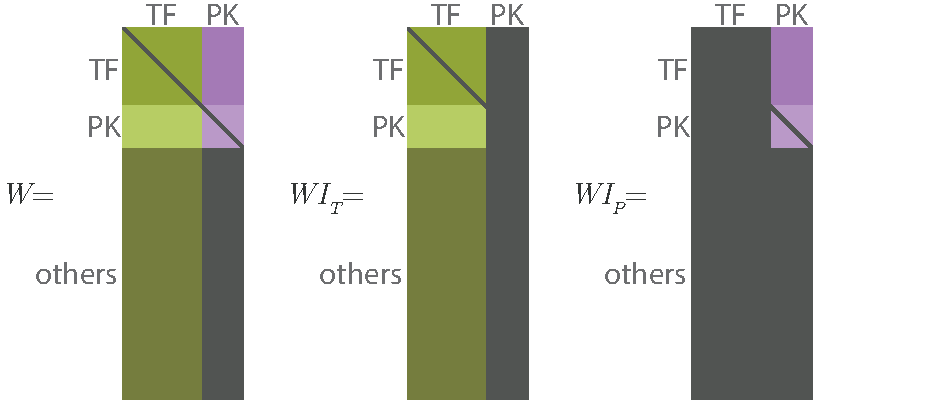
\includegraphics[width=\textwidth]{methods/fig/W.pdf}
    \caption{\textbf{\textit{W}.} Column = edge source, row = target. \\ \textcolor{darkgray}{Dark gray} = 0. Dimensions = $N \times (N_T + N_P)$. }
    \label{fig:W}
\end{figure}
\end{column}
\end{columns}
\end{frame}

\begin{frame}{Equilibrium model}
% Since we are only observing~$\boldsymbol{x}$ we wish to have all other terms for hidden node values disappear which is possible since the model is linear~(\autoref{eq:first_equilibrium_final}).

% If we describe each of the terms as log fold-change versions of absolute measurements for knockout and wildtype experimental conditions, we can get the following~(\autoref{eq:second_equilibrium_def}).
$(t)$ omitted:
\begin{subequations}
\label{eq:second_equilibrium_def}
\begin{equation}
a_i^{(\text{ko})} = y_i^{(\text{ko})} \cdot x_i^{(\text{ko})}
\quad,\quad
a_i^{(\text{wt})} = y_i^{(\text{wt})} \cdot x_i^{(\text{wt})}
\end{equation}\begin{equation}
x_i = \log \frac{x_i^{(\text{ko})}}{x_i^{(\text{wt})}}
\quad,\quad
y_i = \log \frac{y_i^{(\text{ko})}}{y_i^{(\text{wt})}}
\quad,\quad
a_i = \log \frac{a_i^{(\text{ko})}}{a_i^{(\text{wt})}}
= \log \frac{y_i^{(\text{ko})} x_i^{(\text{ko})}}{y_i^{(\text{wt})} x_i^{(\text{wt})}}
= y_i + x_i    
\end{equation}\begin{equation}
\boldsymbol{a}(t) = \boldsymbol{y}(t) + \boldsymbol{x}(t)
\end{equation}
\end{subequations}

% Here $y_i^{(\text{ko})}$ and $y_i^{(\text{wt})}$ are absolute node values, which are typically unmeasured, describing the effective fraction of each protein.

% Owing to the simplicity of a linear model we can cancel out hidden node values as before~(\autoref{eq:second_equilibrium_final}).
Can be shown to converge for $t\rightarrow\infty$
\begin{subequations}
\label{eq:second_equilibrium_final}
\begin{align}
\boldsymbol{a} &= 
    \left(WI_P\boldsymbol{a} + \boldsymbol{e}_y\right) + \boldsymbol{x}
\\
\left(I-WI_P\right) \boldsymbol{a} &=
    \boldsymbol{e}_y + \boldsymbol{x}
\\
\boldsymbol{a} &=
    \left(I-WI_P\right)^{-1} \left(\boldsymbol{e}_y + \boldsymbol{x}\right)
\\
\boldsymbol{x} &=
    WI_T \left(I-WI_P\right)^{-1} \left(\boldsymbol{e}_y + \boldsymbol{x}\right) + \boldsymbol{e}_x
\\
&= WI_T \left(I-WI_P\right)^{-1} \boldsymbol{x} + \boldsymbol{e}
\\
\label{eq:second_equilibrium_final.f}
&= B\boldsymbol{x} + \boldsymbol{e}
\enspace,\enspace B = WI_T \left(I-WI_P\right)^{-1}
\end{align}
\end{subequations}


% Again, the resulting description of observed node values $\boldsymbol{x}$ at equilibrium as a function of itself, can be written as by Eberhardt~et~al. with an extension to $B$. The extension of $B$ is identical to the one at \autoref{eq:first_equilibrium_final.e} with the exception of the 2.
% This model was chosen as the main method going forward based on better intuition in its design, as well as through tests showing little performance difference. 
\end{frame}


\begin{frame}{Equilibrium model - simulation}
\label{sec:prim}

Initial conditions (fig.~\ref{fig:KO_RNA_hist}):
\begin{subequations}
\begin{align}
\boldsymbol{x}_{\mathcal{U}_k} &= 0
\\
\boldsymbol{x}_{\mathcal{J}_k} &\sim \mathcal{N}(\mu=-4, \sigma=1)
\end{align}
\end{subequations}

Simple iteration of eq. \ref{eq:second_equilibrium_final.f} \\
% , where the parameters are chosen based on the observations in . $\boldsymbol{x}(t)$ is then calculated iteratively with \autoref{eq:second_equilibrium_final.f} until approximate convergence is reached, otherwise it will be stopped after 10,000 iterations. Approximate convergence is reached when it holds
Approx. convergence:
\begin{equation}
\label{eq:convergence}
\tfrac{1}{N} \sum_{i=1}^N |x_i(t)-x_i(t-1)| < \epsilon_{tol} \,,\,\epsilon_{tol}=10^{-7}
\end{equation}

\end{frame}

\begin{frame}{Equlibrium model - inference}
\label{sec:equilibrium_inference}

% The obvious way to implement the equations described in \autoref{eq:second_equilibrium_final} in order to infer graph edges will be by applying the algorithm of Eberhardt~et~al., which gives us $B$, and with \autoref{eq:second_equilibrium_final.f} solve for $W$. This cannot be done analytically but is implemented as a gradient descent method where the difference between $B$ and the right hand side of its definition in \autoref{eq:second_equilibrium_final.f} is minimized~(\autoref{eq:loss_B}).
% This approach is referred to as the $B$-method. If there is no covariance matrices for $\boldsymbol{x}_k$ available, $T_{\boldsymbol{x}_k}$ will have to be found using \autoref{eq:t_regress}, which only describes single intervention experiments.

Minimizing a loss function

% Another approach that allows for the inclusion of multiple interventions in an experiment is to minimize~$\boldsymbol{e}$ which is also an attempt at having the least amount of latent variables in the system.
% This approach is referred to as the $\boldsymbol{e}$-minimization method.
% It works by describing the systems of equations from the model in a symbolic math or neural network library in Python. The libraries help by constructing functions for gradients $\dv{\mathcal{L}}{w_{ij}}$, where $\mathcal{L}$ is the loss function and $w_{ij}$ a parameter in $W$. We then minimize the gradient using Adam gradient descent until perceived convergence~\cite{adam}.
% The graph will be sparse which is enforced through L1-regularization. The loss minimized for the $\boldsymbol{e}$-method and $B$-method are:

\begin{subequations}
\label{eq:loss}
\begin{align}
\mathcal{L}_B &=
\sum_{j=1}^N \sum_{i=1}^N
\left(b_{ij} - b_{ij}^{(\text{LLC})}\right)^2
+ \lambda_T \sum_{j \in \text{TF}} \sum_{i=1}^N |w_{ij}| + \lambda_\text{KP} \sum_{j \in \text{KP}} \sum_{i=1}^{N_\text{TF} + N_\text{KP}} |w_{ij}|
\label{eq:loss_B}
\\
\mathcal{L}_{\boldsymbol{e}} &=
\sum_{i=1}^N e_i^2 + \lambda_\text{TF} \sum_{j \in \text{TF}} \sum_{i=1}^N |w_{ij}| + \lambda_\text{KP} \sum_{j \in \text{KP}} \sum_{i=1}^{N_\text{TF} + N_\text{KP}} |w_{ij}|
\label{eq:loss_e}
\end{align}
\end{subequations}

% Here, $\lambda_T$ and $\lambda_P$ are regularization hyperparameters for $W I_T$ and $W I_P$, which means they are chosen to achieve a desired level of sparsity in each of those parts of the weight matrix $W$. They are not necessarily chosen as two different values. $b_{ij}^{(\text{LLC})}$ are values of $B_{\text{LLC}}$ found using LLC. $b_{ij}$ are elements of $B$ which is a function of the trainable parameters in $W$ as described in~\autoref{eq:second_equilibrium_final.f}.


\end{frame}
\subsection{Silent edges}
\begin{frame}{Silent edges}
\label{sec:unobservable}
\begin{columns}
\begin{column}{0.5\textwidth}

\only<1| handout:1>{
Edges silent in RNA logFC data simulated on arbitrary graph

% When inferring a protein-protein or protein-DNA interaction using RNA log fold-change values it is a basic assumption that the RNA values will be affected by the presence or absence of said interaction. In a graph model a TF edge will be observable if the target of the edge is a gene directly measured in the RNA log fold-change data.

% The protein kinases can have outgoing edges with TFs or other PKs as target~(\autoref{fig:unobservable}). If the target of their edge is a TF, then the PK edge will only be detectable if the same can be said for at least one edge from the TF to a measured gene. If the target of the PK edge is another PK, then in order to be detectable, the target will have to have at least one detectable outgoing edge. 


% For real data we will assume that enough genes are recorded that any direct protein-protein or protein-DNA interaction should have some level of effect on gene expression, however small, and that kinase regulation has an effect on gene expression. It is more relevant to consider undetectability for graphs designed artificially from more-or-less random adjacency matrices where it can occur that edges lead to nodes having no outgoing edges themselves.

% A nonsilent node is a node with at least one nonsilent outgoing edge. From a graph with known adjacency matrix $W$ we calculate which nodes are nonsilent with

\begin{equation}
\label{eq:detectable}
\boldsymbol{\omega} =
\sign \sum_{k=0}^K {|W|^\trans}^k
I_T |W|^\trans \boldsymbol{1} 
\end{equation}
\begin{conditions}
|W| & element-wise absolute of $W$ \\
\boldsymbol{1} & vector of 1s
\end{conditions}
% Here $\boldsymbol{\omega}$ is a vector where entry $\omega_i$ will be 1 if node $i$ is detectable and 0 otherwise. The superscript $\trans$ refers to transposing. $W$ has to be square, which it is in all cases where this equation has been applied. $\sign$ is the sign function, $|W|$ is the absolute of $W$, $\boldsymbol{1}$ is a vector of 1s with length $N_T + N_P$. $K$ is the length of the longest cascade of protein kinases, which is found through iterative calculation of $\boldsymbol{\omega}(K)$ as the smallest $K$ for which it holds that $\boldsymbol{\omega}(K) = \boldsymbol{\omega}(K + 1)$.


% \autoref{eq:detectable} can be read as starting with finding all TFs with at least one outgoing edges~($W^\trans \boldsymbol{1} I_T$), and iteratively follow all kinase cascades backwards for each iteration $k$.
}

\only<2| handout:2>{

% The simple network in~\autoref{fig:unobservable} can be used as an example, where we assign some random positive and negative values to each edge. Columns and rows in $W$ are sorted with TF first and PK second, so the order is $\text{TF}_1,\text{TF}_2,\text{TF}_3,\text{PK}_1,\text{PK}_2,\text{PK}_3$.

\begin{subequations}
\begin{align*}
\label{eq:detectable_example}
W &=
\begin{bmatrix} 
0 & 0 & 0 & 0 & 0 & -0.8 \\
0 & 0 & 0 & 0 & 0 & 0.7 \\
0 & 0 & 0 & 0 & -0.1 & 0.3 \\
1.1 & 0 & 0 & 0 & 0 & -0.4 \\
0 & 0 & 0 & 0 & 0 & 0 \\
0 & 0 & 0 & 0 & 0.5 & 0 \\
\end{bmatrix}
\\
|W|^\trans &=
\begin{bmatrix} 
0 & 0 & 0 & 1.1 & 0 & 0 \\
0 & 0 & 0 & 0 & 0 & 0 \\
0 & 0 & 0 & 0 & 0 & 0 \\
0 & 0 & 0 & 0 & 0 & 0 \\
0 & 0 & 0.1 & 0 & 0 & 0.5 \\
0.8 & 0.7 & 0.3 & 0.4 & 0 & 0 \\
\end{bmatrix}
\end{align*}
\end{subequations}

}


\only<3| handout:3>{

\begin{subequations}
\begin{align*}
I_T |W|^\trans \boldsymbol{1}
=
\sum_{k=0}^0 {|W|^\trans}^k
I_T |W|^\trans \boldsymbol{1}
&=
\begin{bmatrix} 
1.1 \\
0 \\
0 \\
0 \\
0 \\
0 \\
\end{bmatrix}
\\
\sum_{k=0}^1 {|W|^\trans}^k
I_T |W|^\trans \boldsymbol{1}
&=
\begin{bmatrix} 
1.1 \\
0 \\
0 \\
0 \\
0 \\
0.88 \\
\end{bmatrix}
\end{align*}
\end{subequations}

}

\only<4| handout:4>{

\begin{subequations}
\begin{align*}
\sum_{k=0}^2 {|W|^\trans}^k
I_T |W|^\trans \boldsymbol{1}
&=
\begin{bmatrix} 
1.1 \\
0 \\
0 \\
0 \\
0.44 \\
0.88 \\
\end{bmatrix}
\\
\sum_{k=0}^3 {|W|^\trans}^k
I_T |W|^\trans \boldsymbol{1}
&=
\begin{bmatrix} 
1.1 \\
0 \\
0 \\
0 \\
0.44 \\
0.88 \\
\end{bmatrix}
\end{align*}
\end{subequations}
}
\only<5| handout:5>{
% There is no change in the calculation from $K=2$ to $K=3$ so we set $K$ equal to 2 and get
\begin{equation*}
\label{eq:silent_example}
\boldsymbol{\omega} = \begin{bmatrix} 
1 \\
0 \\
0 \\
0 \\
1 \\
1 \\
\end{bmatrix}
\quad,\quad
M_s =
\begin{bmatrix} 
1 & 1 & 1 & 1 & 1 & 1 \\
1 & 1 & 1 & 0 & 0 & 0 \\
1 & 1 & 1 & 0 & 0 & 0 \\
1 & 1 & 1 & 0 & 0 & 0 \\
1 & 1 & 1 & 1 & 1 & 1 \\
1 & 1 & 1 & 1 & 1 & 1 \\
\end{bmatrix}
\end{equation*}
% This means that $\text{TF}_2,\text{TF}_3,\text{PK}_1$ are silent nodes. From $\boldsymbol{\omega}$ we can find the set of silent edges, which are all activity regulating edges onto any of the silent nodes. These entries in $W$ of silent edge is shown as zeros in $M_S$~(\autoref{eq:silent_example}), which is the masking matrix that indicates the edges to consider for a performance evaluation on an edge inference attempt. It is clear to spot the four edges in $W$ that are too be ignored if we were to infer edges for this network.
}
\stepcounter{equation}
\end{column}
\begin{column}{0.5\textwidth}
\begin{figure}[ht]
    \centering
    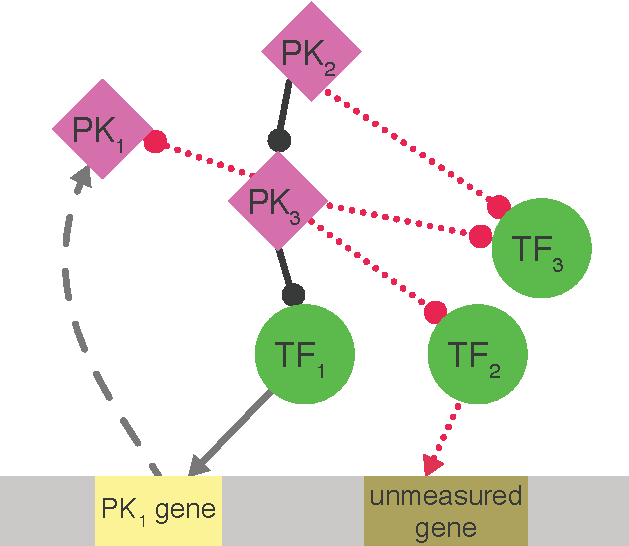
\includegraphics[width=0.6\textwidth]{theory/fig/unobservable.pdf}
    \caption{\textbf{Silent edges.} \textcolor{red}{red} = silent, \textcolor{black}{black} = detectable PK edge, dashed = transcription/translation, \textcolor{darkgray}{dark gray} = TF edge. }
    \label{fig:unobservable}
\end{figure}

\end{column}
\end{columns}
\end{frame}

\begin{frame}{Silent edges - removing $K$}
% As mentioned, $K$ in~\autoref{eq:detectable} is the length of the longest kinase cascade, or more precisely, the iteration where, if we computed further iterations of the sum, it would not change $\boldsymbol{\omega}$. We can simplify by letting $K$ tend to infinity.
for $K\rightarrow\infty$
\begin{equation}
\boldsymbol{\omega} =
\sign \sum_{k=0}^\infty {|W|^\trans}^k
I_T |W|^\trans \boldsymbol{1}
=
\sign \left( \left( \sum_{k=0}^\infty {|W|^\trans}^k \right)
I_T |W|^\trans \boldsymbol{1} \right)
\end{equation}
% If $I-|W|^\trans$ is invertible we can simplify the sum, using the same rule applied by Eberhardt~et~al.~(\autoref{eq:eber_converge.b}). We assume this holds since our system~(\autoref{eq:basic_eberhardt_extension}) is meant to reach equilibrium. It will not be assumed to hold for "gold standard" matrices discussed later~(\autoref{sec:dream_data}), since these does not hold edge values before preprocessing, and would diverge if used as such.
Simplify using same rule applied by Eberhardt~et~al.~(eq.~\ref{eq:eber_converge})
\begin{equation}
\label{eq:detectable_no_K}
\boldsymbol{\omega} =
\sign \left( \left( I - {|W|^\trans} \right)^{-1}
I_T |W|^\trans \boldsymbol{1} \right)
\end{equation}
% \autoref{eq:detectable_no_K} was tested on $W$ given in \autoref{eq:detectable_example}, which as expected produced $\boldsymbol{\omega}$ from \autoref{eq:silent_example} (a tolerance of $>\num{1e-14}$ was used instead of $\sign$ due to the imperfect nature of floating-point computation).
\end{frame}






% \begin{frame}{Convergence model}
\label{sec:convergence_model}

% A convergence model was tested, where, instead of formulas describing a system at equilibrium, the system's nonlinear dynamics can be formulated and simulated until approximate convergence. It allows the model to have large amounts of nonlinearity but increases calculation costs significantly.

% A machine learning model was formulated to mimic gene regulation~(\autoref{eq:convergence_model}). It was designed for pseudo-simulation of a wildtype expression converging to the observed RNA expression levels for mutants. The equations described here applies iterative calculation of protein kinase activity for signal cascades, where after $k_{\max}$ iterations the protein kinase activities~$\boldsymbol{a}_P(t,k)$ are used for calculations of transcription factor activities~$\boldsymbol{a}_T(t)$, which are used for calculating predicted gene expression levels~$\boldsymbol{x}(t)$. The loss function $\mathcal{L}_C$ is then formulated as the sum of squared errors of the gene expression prediction $\boldsymbol{x}(t=t_{\max})$ and the measured gene expression levels $y$. Lastly, a L1-regularization is applied on the trainable parameters of the model.

\begin{subequations}
\label{eq:convergence_model}
\begin{align}
\boldsymbol{a}_P (t=0,k=0) &= \boldsymbol{c}_P
\quad,\quad
\boldsymbol{x}(t=0) = \boldsymbol{0}
\\
\boldsymbol{a}_P (t>0,k=0) &= \boldsymbol{a}_P (t-1,k=k_{\max})
\\
\boldsymbol{a}_P (t>0,k>0) &=
U_P \tanh \left(W_{PP} \boldsymbol{a}_P(t,k-1) + M_P \boldsymbol{x}(t-1) \right) + \boldsymbol{c}_P
\\
\boldsymbol{a}_T (t) &=
U_T \tanh \left(W_{PT} \boldsymbol{a}_P(t,k=k_{\max}) + M_T \boldsymbol{x}(t-1) \right) + \boldsymbol{c}_T
\\
\boldsymbol{x}(t) &= \tanh(W_{TX} \boldsymbol{a}_T(t))
\\
\mathcal{L}_C &= \left(\boldsymbol{x}(t=t_{\max}) - \boldsymbol{y}\right)^2
+ \lambda \left(\sum_{j=1}^{N_P}\sum_{i=1}^{N_P}|w_{ij}^{(PP)}| + \sum_{j=1}^{N_P}\sum_{i=1}^{N_T}|w_{ij}^{(PT)}| + \sum_{j=1}^{N_T}\sum_{i=1}^{N}|w_{ij}^{(TX)}| \right)
\end{align}
\end{subequations}
\begin{conditions}
t & time step \\
k & PK cascade step \\
\boldsymbol{x}(t), \boldsymbol{y} & predicted and measured gene expression \\
\boldsymbol{a}_P(t,k), \boldsymbol{a}_T(t) & activity relative to WT for PK, and TF \\
U_P, U_T & mask knocked out PK, and TF \\
\boldsymbol{c}_P, \boldsymbol{c}_T & intervention for PK, and TF \\
M_P, M_T & map gene to product \\
W_{PP}, W_{PT}, W_{TX} & trainable weights
\end{conditions}
% Here, $t$, and $k$ refers to discrete timesteps of gene production and iteration of PK cascade, respectively. $\boldsymbol{a}_P(t,k)$, and $\boldsymbol{a}_T(t,k)$ are activities of protein kinases relative to wildtype. $U_P$, and $U_T$ are masking matrices, removing values of knocked out genes, similar to $U_k$ from~\autoref{sec:eberhardt}. $\boldsymbol{c}_P$ and $\boldsymbol{c}_T$ are vectors of zeros except for indices of knockouts where they are arbitrarily set to -1 to indicate fully reduced activity. Since $\tanh$ is used, all values will be in range $[-1,1]$. $M_P$, and $M_T$ are masking arrays with ones mapping gene indices to their respective protein product indices. $W_{PP}$, $W_{PT}$, and $W_{TX}$ are trainable weight parameters for PK$\rightarrow$PK, PK$\rightarrow$TF, and TF$\rightarrow$gene interactions. $N_P$ is the number of PKs, $N_T$ the number TFs, and $N$ the total count of all genes measured, including TFs, and PKs.

% This model has high computational cost, the formulas are not biologically intuitive, and the model can be criticized for the expectation that convergence is assumed to be reached within a small finite number of iterations. It would be possible to design a model where $\boldsymbol{x}$ is not reset for each gradient descent step, and to allow time $t$ to increase through the entirety of training, however this is beyond what has been tested here.

% Convergence models were initially tested, both with SGD~(Stochastic Gradient Descent), Adam gradient descent, an evolutionary algorithm of learning parameters. A concern was whether the training would be too costly to run. It was found that it was not too costly when testing with Theano or PyTorch, but that error convergence was inadequate for the data in~\autoref{sec:yeast_data}, but perfect for small testing datasets. The equilibrium model is simpler and creates better intuition so the convergence model is not documented in~\autoref{sec:analysis}.
\end{frame}





